% !TEX TS-program = pdflatex
% !TEX encoding = UTF-8 Unicode

% This is a simple template for a LaTeX document using the "article" class.
% See "book", "report", "letter" for other types of document.

\documentclass[12pt]{article} % use larger type; default would be 10pt

\usepackage[utf8]{inputenc} % set input encoding (not needed with XeLaTeX)

%%% Examples of Article customizations
% These packages are optional, depending whether you want the features they provide.
% See the LaTeX Companion or other references for full information.

%%% PAGE DIMENSIONS
\usepackage{geometry} % to change the page dimensions
\geometry{a4paper} % or letterpaper (US) or a5paper or....
\geometry{margin=1in} % for example, change the margins to 2 inches all round
% \geometry{landscape} % set up the page for landscape
%   read geometry.pdf for detailed page layout information

\usepackage{graphicx} % support the \includegraphics command and options

%%% PACKAGES
\usepackage{booktabs} % for much better looking tables
\usepackage{array} % for better arrays (eg matrices) in maths
\usepackage{paralist} % very flexible & customisable lists (eg. enumerate/itemize, etc.)
\usepackage{verbatim} % adds environment for commenting out blocks of text & for better verbatim
%\usepackage{subfig} % make it possible to include more than one captioned figure/table in a single float
\usepackage{amsmath,mathtools,amsfonts}
\usepackage{bm}
\usepackage{blindtext}
\usepackage{fancyhdr}
\usepackage{float}
\usepackage{gensymb}
\usepackage{svg}
\usepackage{subcaption}
\usepackage{listings}
\usepackage{color}
\usepackage[justification=centering]{caption}
\usepackage[utf8]{inputenc}
\usepackage{pgfplotstable,filecontents}
\usepackage{csvsimple}
\usepackage{pdfpages}

\definecolor{mygreen}{rgb}{0,0.6,0}
\definecolor{mygray}{rgb}{0.5,0.5,0.5}
\definecolor{mymauve}{rgb}{0.58,0,0.82}

\lstset{ 
	backgroundcolor=\color{white},   % choose the background color; you must add \usepackage{color} or \usepackage{xcolor}; should come as last argument
	basicstyle=\footnotesize,        % the size of the fonts that are used for the code
	breakatwhitespace=false,         % sets if automatic breaks should only happen at whitespace
	breaklines=true,                 % sets automatic line breaking
	captionpos=b,                    % sets the caption-position to bottom
	commentstyle=\color{mygreen},    % comment style
	deletekeywords={...},            % if you want to delete keywords from the given language
	escapeinside={\%*}{*)},          % if you want to add LaTeX within your code
	extendedchars=true,              % lets you use non-ASCII characters; for 8-bits encodings only, does not work with UTF-8
	firstnumber=001,                % start line enumeration with line 1000
	frame=single,	                   % adds a frame around the code
	keepspaces=true,                 % keeps spaces in text, useful for keeping indentation of code (possibly needs columns=flexible)
	keywordstyle=\color{blue},       % keyword style
	language=Octave,                 % the language of the code
	morekeywords={*,...},            % if you want to add more keywords to the set
	numbers=left,                    % where to put the line-numbers; possible values are (none, left, right)
	numbersep=5pt,                   % how far the line-numbers are from the code
	numberstyle=\tiny\color{mygray}, % the style that is used for the line-numbers
	rulecolor=\color{black},         % if not set, the frame-color may be changed on line-breaks within not-black text (e.g. comments (green here))
	showspaces=false,                % show spaces everywhere adding particular underscores; it overrides 'showstringspaces'
	showstringspaces=false,          % underline spaces within strings only
	showtabs=false,                  % show tabs within strings adding particular underscores
	stepnumber=2,                    % the step between two line-numbers. If it's 1, each line will be numbered
	stringstyle=\color{mymauve},     % string literal style
	tabsize=2,	                   % sets default tabsize to 2 spaces
	title=\lstname                   % show the filename of files included with \lstinputlisting; also try caption instead of title
}

\graphicspath{ {./images/}{../graphs/} }

%%% HEADERS & FOOTERS
\pagestyle{fancy}
\renewcommand{\headrulewidth}{1pt} % customise the layout...
\renewcommand{\footrulewidth}{1pt} % customise the layout...
\fancyhf{}

% HEADER
\fancyhead[L]{Will Cowper (81163265)}
\fancyhead[C]{}
\fancyhead[R]{Jesse Sheehan (53366509)}

% FOOTER
\fancyfoot[L]{}
\fancyfoot[C]{\thepage}
\fancyfoot[R]{}

%% TITLE
\title{\uppercase{
	Flow Planning\\
	\large{Assignment 2} \\
	\small{COSC364-19S1 Internet Technology and Engineering}
}}
\date{\today}
\author{
	Will Cowper\\
	{\small{ID: 81163265}}\\
	{\small{Contribution: 50\%}}\\
	\\
	Jesse Sheehan\\
	{\small{ID: 53366509}}\\
	{\small{Contribution: 50\%}}\\
	\\
}

\begin{document}

\maketitle

\begin{figure}[H]
	\centering
	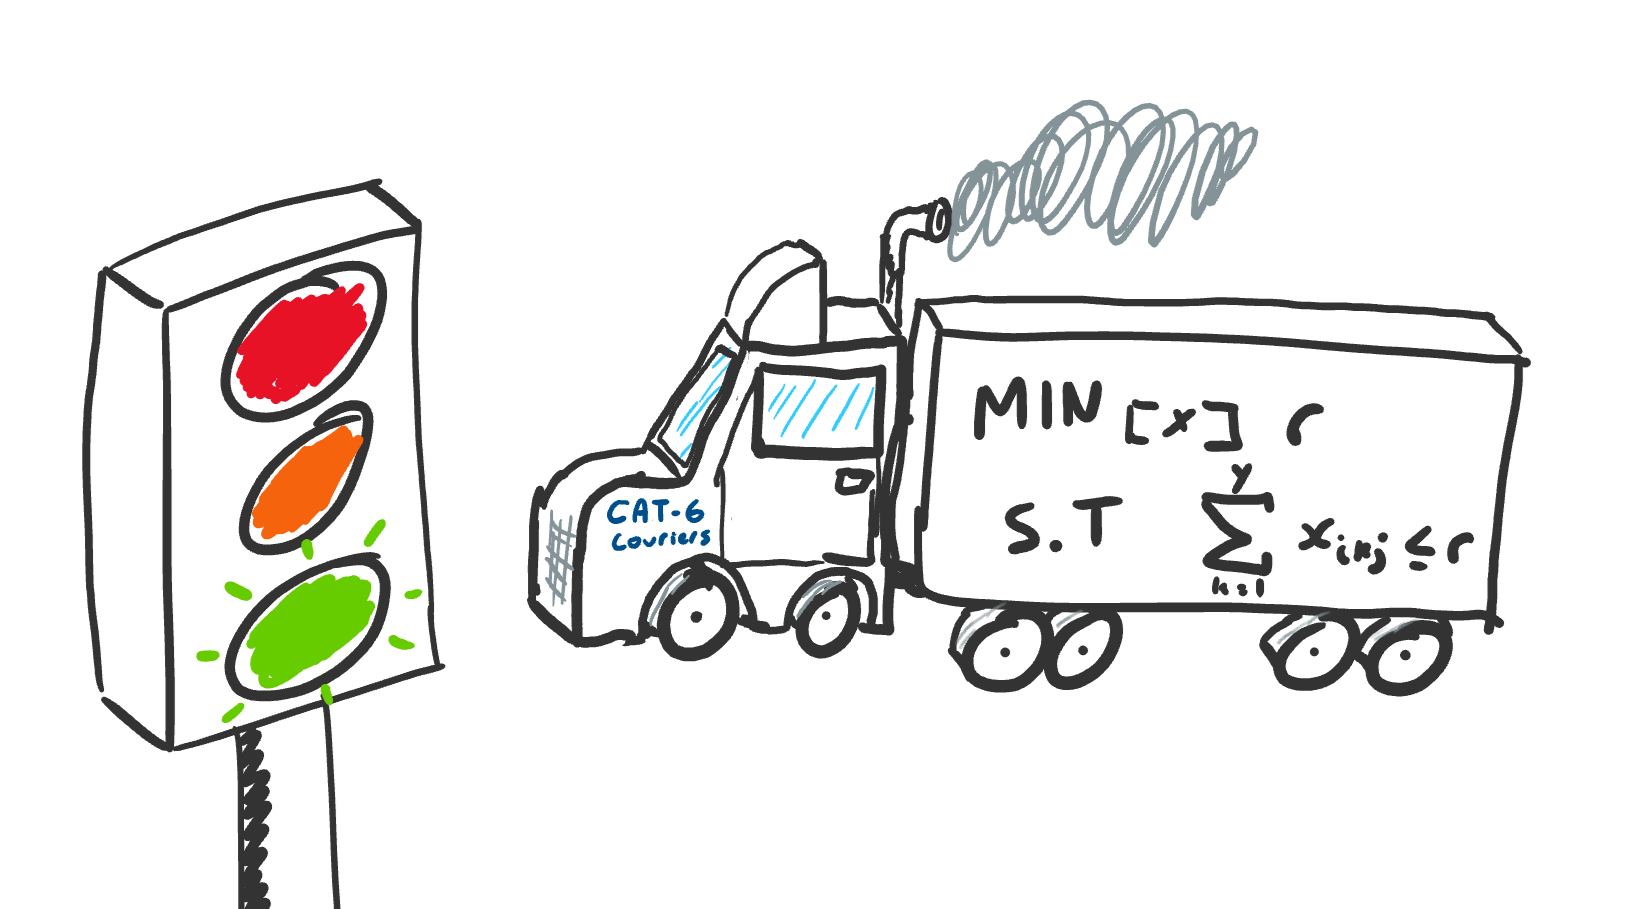
\includegraphics[width=\textwidth]{traffic}
	\caption{Traffic problems are not unique to computer networks.}
	\label{fig:traffic}
\end{figure}

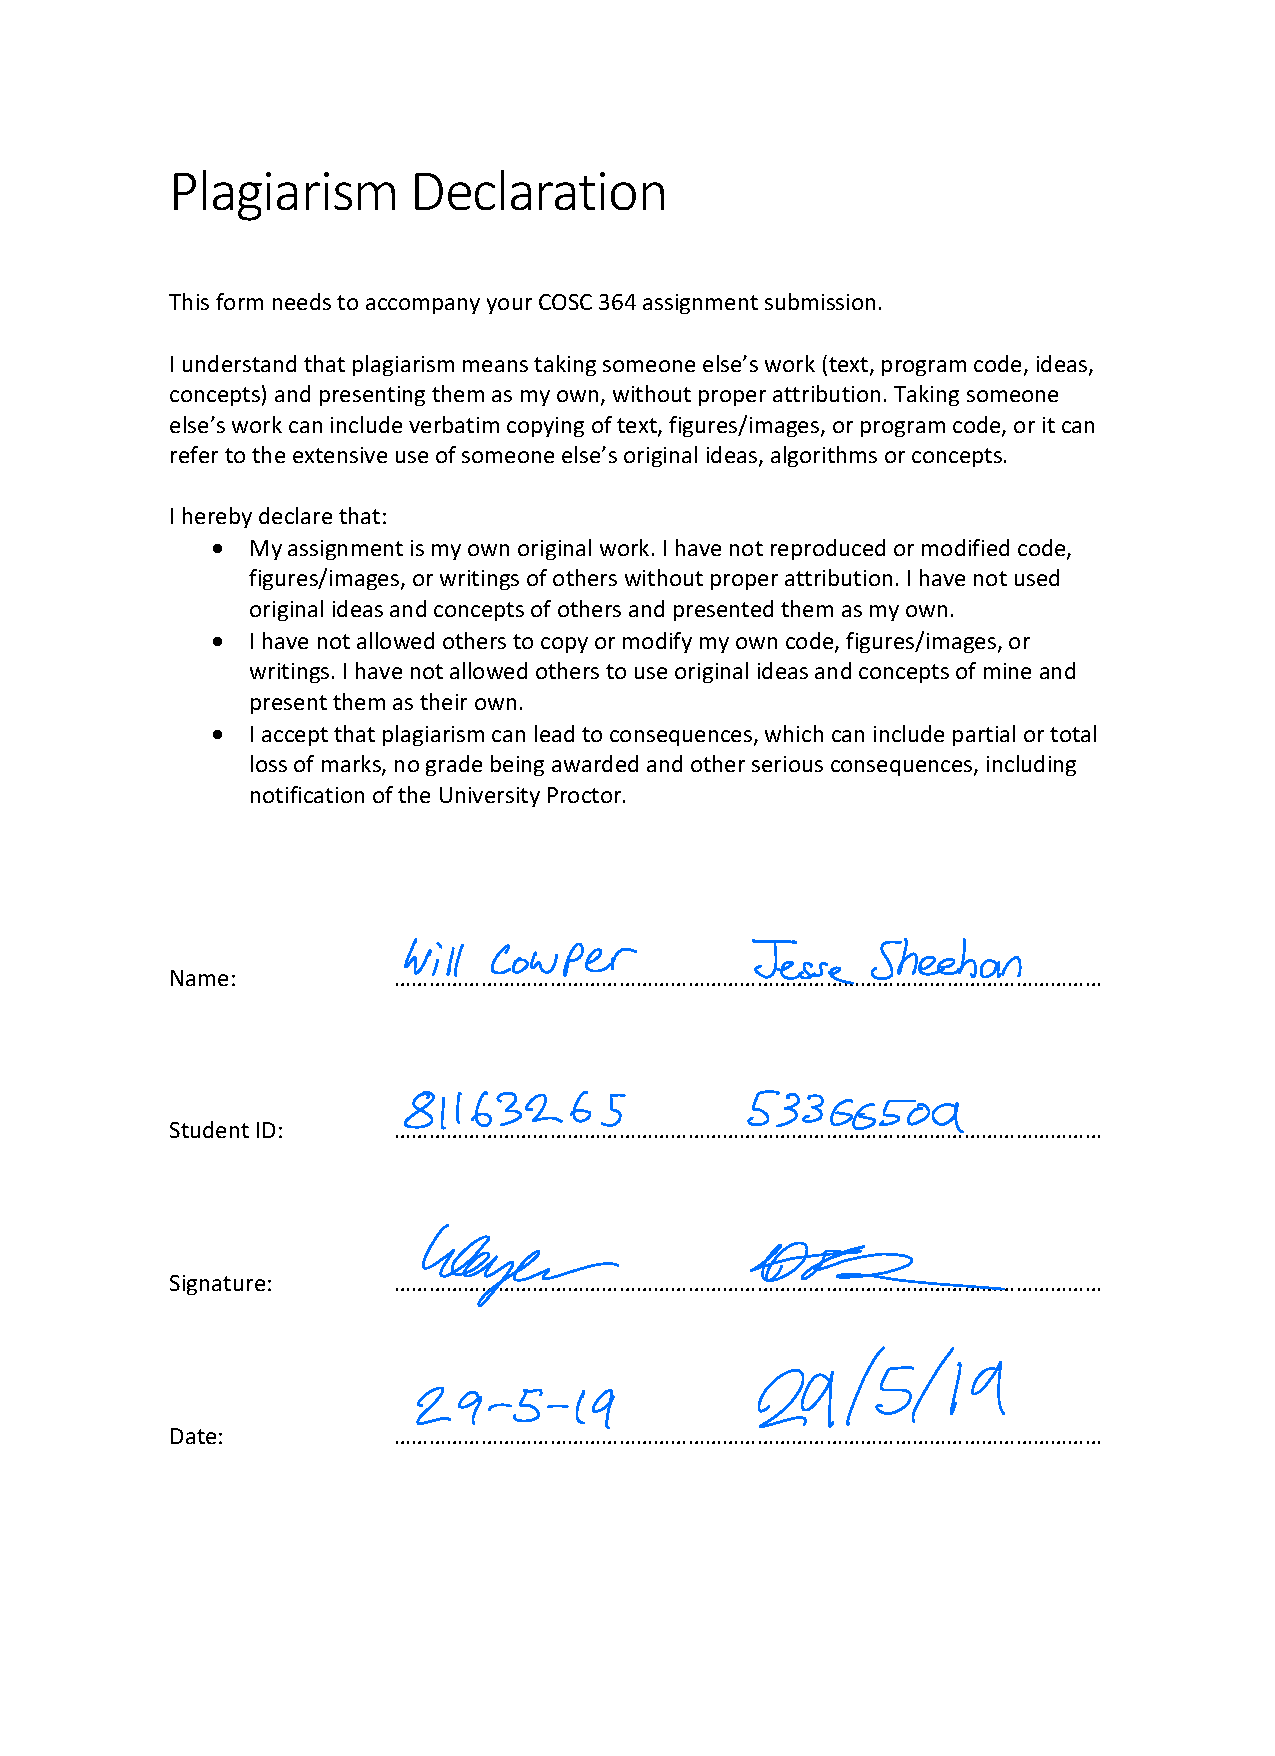
\includepdf{includes/plagiarism_declaration.pdf}

\section{Problem Description}

Given a network (figure \ref{fig:network}) with $X$ source nodes, $Y$ transit nodes and $Z$ destination nodes, a program was designed to generate an LP file that could be used by CPLEX to determine certain network characteristics.

\begin{figure}[H]
	\centering
	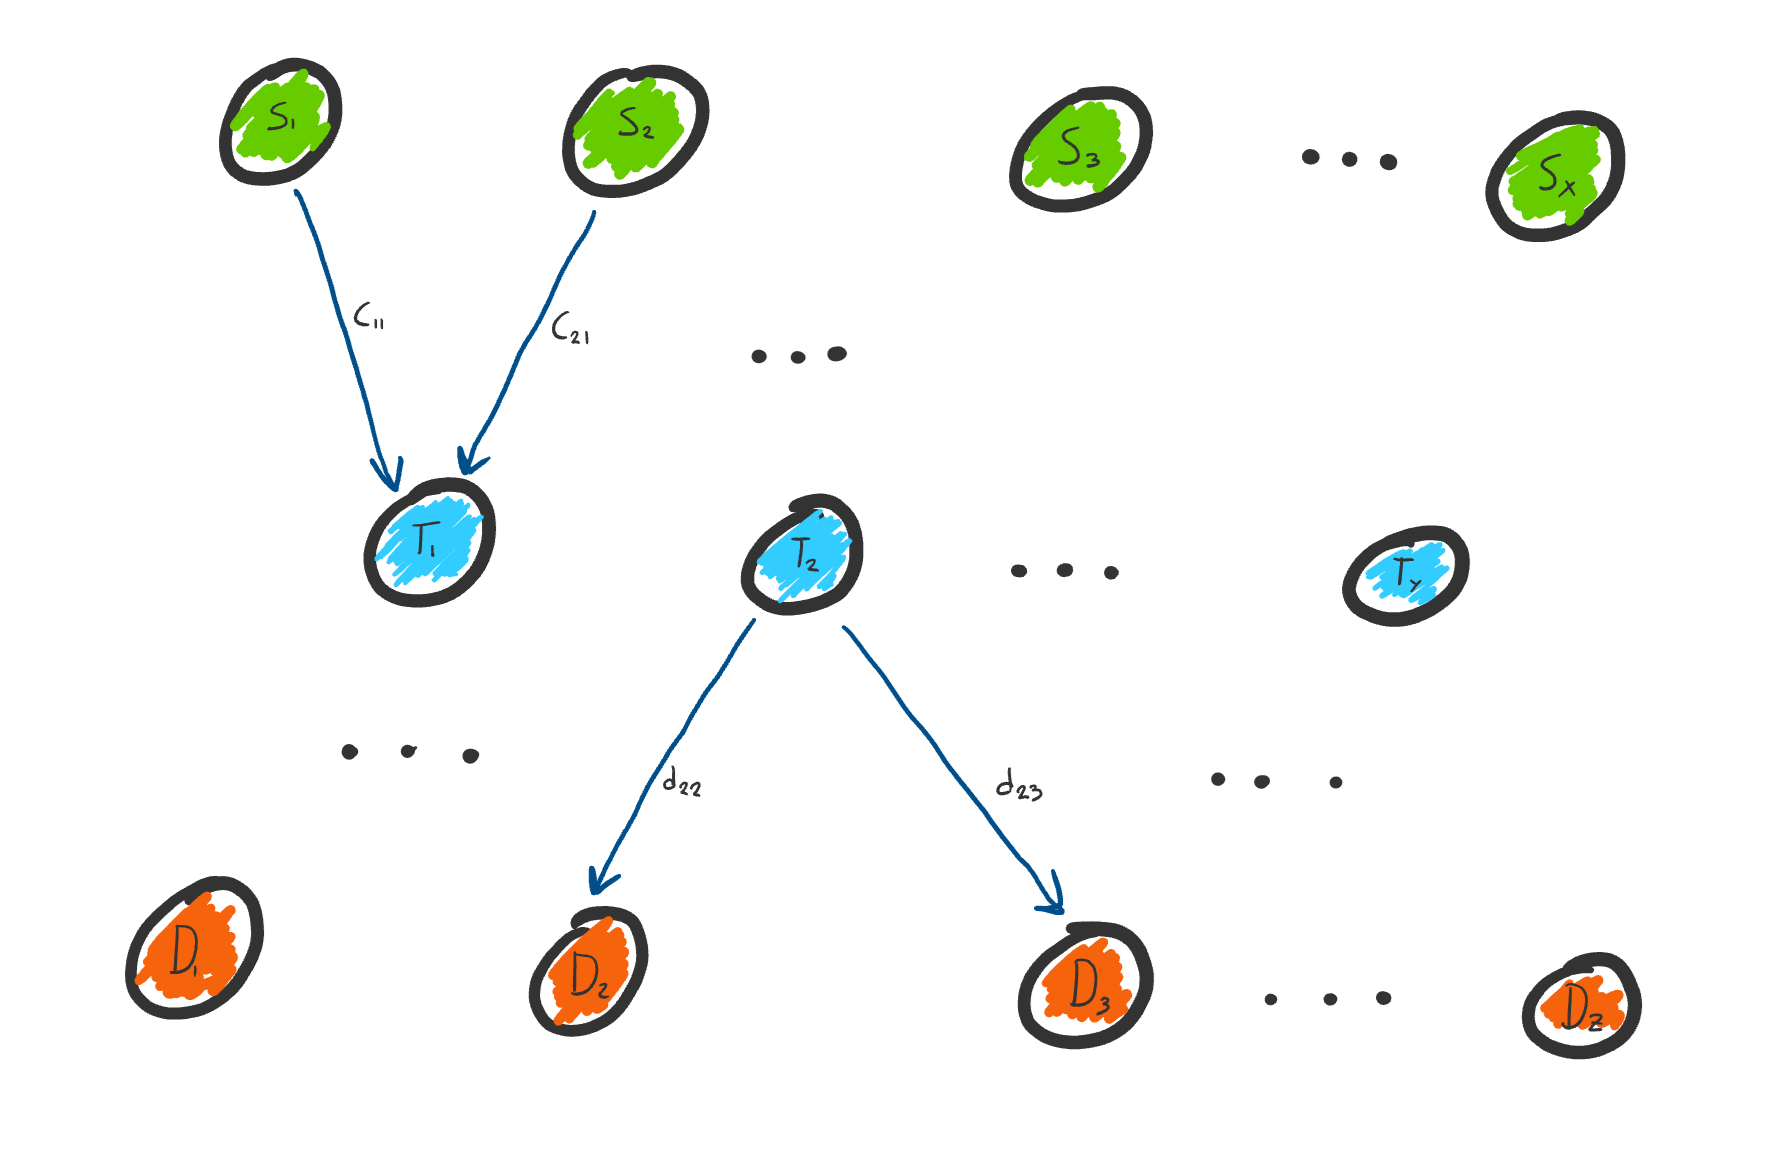
\includegraphics[width=\textwidth]{network}
	\caption{An example network showing nodes $S_i$, $T_k$ and $D_j$ and links $c_{ik}$ and $d_{kj}$, $i \in \{1, \ldots, X\}, k \in \{1, \ldots, Y\}, j \in \{1, \ldots, Z\}$.}
	\label{fig:network}
\end{figure}

Traffic travelling from $S_i$ to $D_j$ must travel through exactly 2 transit nodes with a total demand volume of $h_{ij}$ (equation \ref{eq:demand_definition}). Furthermore, the load upon each transit node must be balanced.

\section{Problem Formulation}

\noindent This problem was solved with the use of binary variable constraints (equations \ref{eq:binary_select_constraint}, \ref{eq:binary_constraint} and \ref{eq:binary_definition}) and the minimisation of our objective function (equation \ref{eq:obj_func_def}).
All normal non-negativity constraints were applied (equations \ref{eq:obj_function_nn}, \ref{eq:decision_var_nn}, \ref{eq:source_capacity_nn} and \ref{eq:dest_capacity_nn}).\\

\noindent The following network properties were solved for:
\begin{itemize}
	\item The capacities of each link (equations \ref{eq:source_capacity_constraint} and \ref{eq:dest_capacity_constraint}).
	\item The load on each transit node (equation \ref{eq:transit_link_capacity_constraint}).
	\item The value of each flow (equations \ref{eq:demand_flow_constraint} and \ref{eq:decision_var_constraint}).
\end{itemize}

\newpage

\noindent \textbf{Notation:}
\begin{itemize}
\item $X$ is the number of source nodes.
\item $Y$ is the number of transit nodes.
\item $Z$ is the number of destination nodes.
\item $S_i$ is the $i$th source node.
\item $T_k$ is the $k$th transit node.
\item $D_j$ is the $j$th destination node.
\item $h_{ij}$ is the demand flow between $S_i$ and $D_j$. This is equal to $2i + j$.
\item $c_{ik}$ is the link capacity between $S_i$ and $T_k$.
\item $d_{kj}$ is the link capacity between $T_k$ and $D_j$.
\item $x_{ikj}$ is the decision variable associated with the path $S_i$-$T_k$-$D_j$.
\item $u_{ikj}$ is the binary decision variable associated with $x_{ikj}$. These are required because $h_{ij}$ must be split across exactly 2 transit nodes.
\item $l_{k}$ is the load on $T_k$.
\end{itemize}

\noindent \textbf{Note:} Due to the limitations of the LP file format, many of the following equations must be rearranged for use in CPLEX. Most notably, there cannot be any variables on the right hand side of an equality or inequality. \\

\noindent Python, BASH and PowerShell scripts (section \ref{section:source}) were used to automate the process (figure \ref{fig:scriptflow}) of generating the LP files, analysing the CPLEX data, and producing graphs.

\begin{figure}[H]
	\centering
	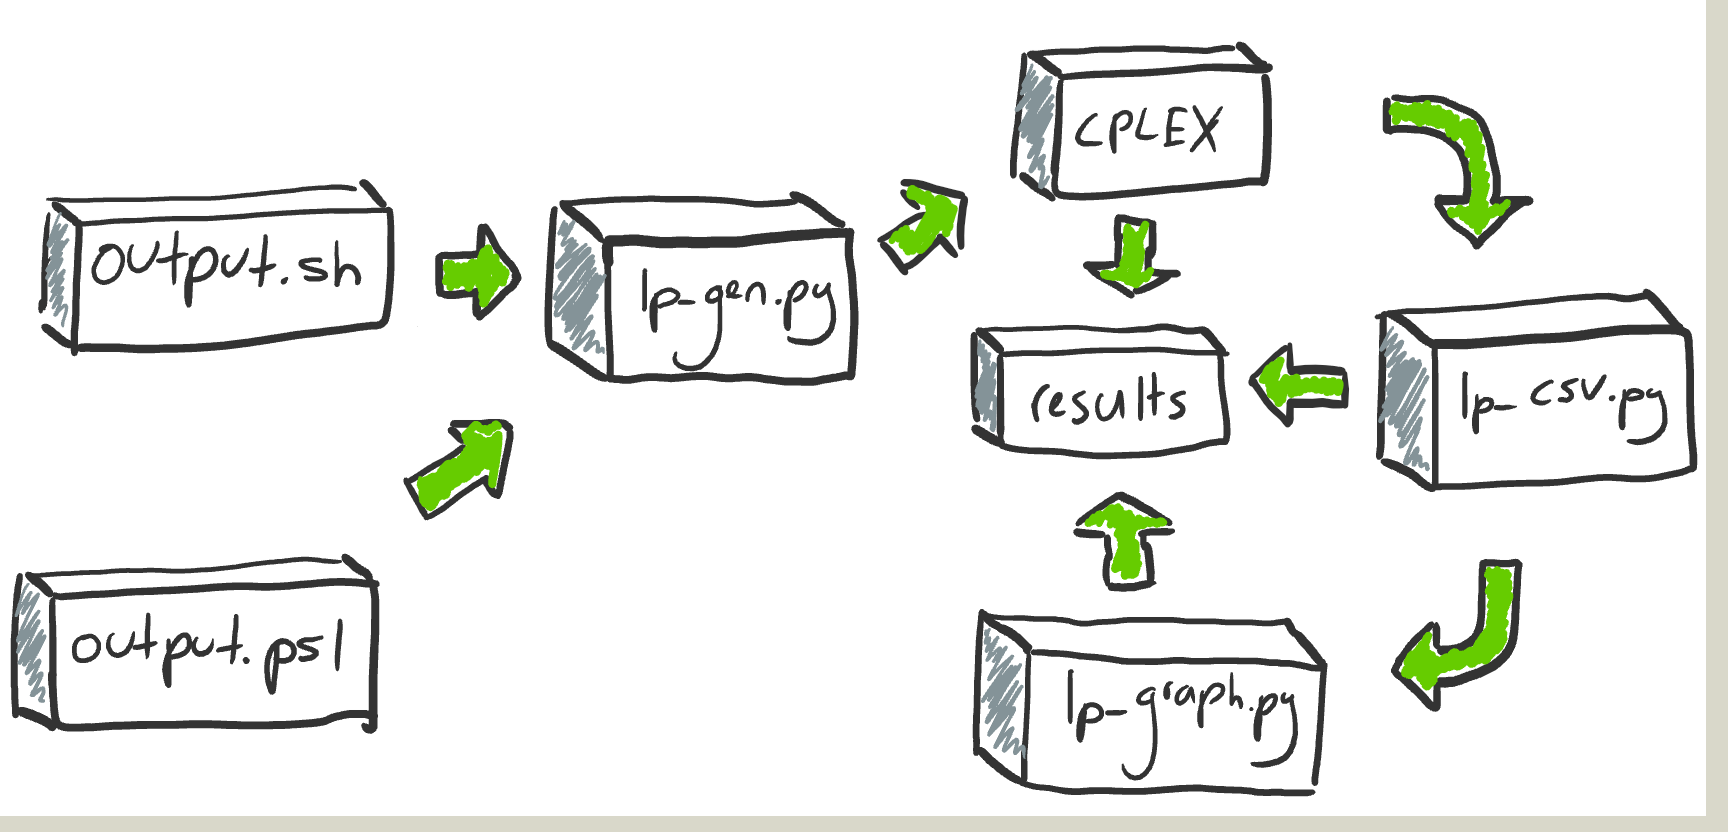
\includegraphics[width=\textwidth]{scriptflow}
	\caption{A graphical interpretation of the script execution used.}
	\label{fig:scriptflow}
\end{figure}

\newpage

\subsection{Objective Function}

\begin{align}
\label{eq:obj_func_def}
\text{minimize}_{[x, c, d, r]}\ r
\end{align}

\subsection{Constraints}

\begin{align}
\label{eq:demand_flow_constraint}
\sum_{k = 1}^{Y} x_{ikj} &= h_{ij} & i \in \{1, \ldots, X\}, j \in \{1, \ldots, Z\} \\[1em]
\label{eq:source_capacity_constraint}
\sum_{j = 1}^{Z} x_{ikj} &= c_{ik} & i \in \{1, \ldots, X\}, k \in \{1, \ldots, Y\} \\[1em]
\label{eq:dest_capacity_constraint}
\sum_{i = 1}^{X} x_{ikj} &= d_{kj} & k \in \{1, \ldots, Y\}, j \in \{1, \ldots, Z\} \\[1em]
\label{eq:transit_link_capacity_constraint}
\sum_{k = 1}^{Y} x_{ikj} &= l_k & i \in \{1, \ldots, X\}, j \in \{1, \ldots, Z\} \\[1em]
\label{eq:binary_select_constraint}
\sum_{k = 1}^{Y} u_{ikj} &= 2 & i \in \{1, \ldots, X\}, j \in \{1, \ldots, Z\} \\[1em]
\label{eq:binary_constraint}
x_{ikj} &= \frac{u_{ikj}h_{ij}}{2} & i \in \{1, \ldots, X\}, k \in \{1, \ldots, Y\}, j \in \{1, \ldots, Z\} \\[1em]
\label{eq:decision_var_constraint}
\sum_{i = 1}^{X} \sum_{j = 1}^{Z} x_{ikj} &\leq r & k \in \{1, \ldots, Y\} \\[1em]
\label{eq:binary_definition}
u_{ikj} &\in \{0, 1\} & i \in \{1, \ldots, X\}, k \in \{1, \ldots, Y\}, j \in \{1, \ldots, Z\} \\[1em]
\label{eq:demand_definition}
h_{ij} &= 2i + j & i \in \{1, \ldots, X\}, j \in \{1, \ldots, Z\}
\end{align}

\subsection{Non-Negativity Constraints}

\begin{align}
\label{eq:obj_function_nn}
r &\geq 0 \\[1em]
\label{eq:decision_var_nn}
x_{ikj} &\geq 0 & i \in \{1, \ldots, X\}, k \in \{1, \ldots, Y\}, j \in \{1, \ldots, Z\} \\[1em]
\label{eq:source_capacity_nn}
c_{ik} &\geq 0 & i \in \{1, \ldots, X\}, k \in \{1, \ldots, Y\} \\[1em]
\label{eq:dest_capacity_nn}
d_{kj} &\geq 0 & k \in \{1, \ldots, Y\}, j \in \{1, \ldots, Z\}
\end{align}

\section{Results}

LP files were generated with parameters $X = Z = 9, Y \in \{3, 4, 5, 6, 7, 8\}$. These were then processed with CPLEX, recording the time taken to solve each problem. Important data points were extracted from the CPLEX output and are listed in table \ref{tab:results}.

\begin{table}[H]
	\centering
	\caption{The raw data as extracted and processed from the CPLEX output.}
	\csvautotabular[table head=\hline \textbf{Y} & \textbf{Time (ms)} & \textbf{Links} & \textbf{Load Spread} & \textbf{Max. $\bf{c_{ik}}$} & \textbf{Max. $\bf{d_kj}$}\\ \hline \csvlinetotablerow\\]{../lp_files/cplex_data.csv}
	\label{tab:results}
\end{table}

\noindent An analysis of these results confirms many assumptions that were made about the problem. The number of non-zero link capacities increases linearly (figure \ref{fig:cplex_num_nonzero_links}), the transit node load spread is very close to (if not exactly) zero for most networks (figure \ref{fig:cplex_transit_load_spread}), and the amount of time taken to solve the problem increases (almost) non-linearly as the number of transit nodes increases (figure \ref{fig:cplex_time}). It is important to note that the load on the transit nodes was only able to be balanced in three of the networks, however the load spread on the remaining three networks is very low. CPLEX has done its best to equalise the loads on each transit node but could not balance them in some cases due to the demand flows and the number of nodes. \\

\noindent The most obvious feature of the results is the data for the $Y=7$ network. It appears to be an outlier as it takes less time to solve than the $Y=5$ and $Y=6$ networks and has the highest transit node load spread by a factor of 3. \textbf{Explain this behaviour!!!} \\

\noindent The second odd feature of the data is the greatest link capacities of the $Y=3$ and $Y=6$ networks (figure \ref{fig:cplex_highest_capacity_links}). The exact reason behind this behaviour is unknown but it would have something to do with these specific combinations of $X$, $Y$ and $Z$ not being relatively prime. % AKA BLACK MAGIC FUCKERY
% MAYBE ANSWER THIS PROPERLY INSTEAD OF SPINNING A YARN

\begin{figure}[H]
	\centering
	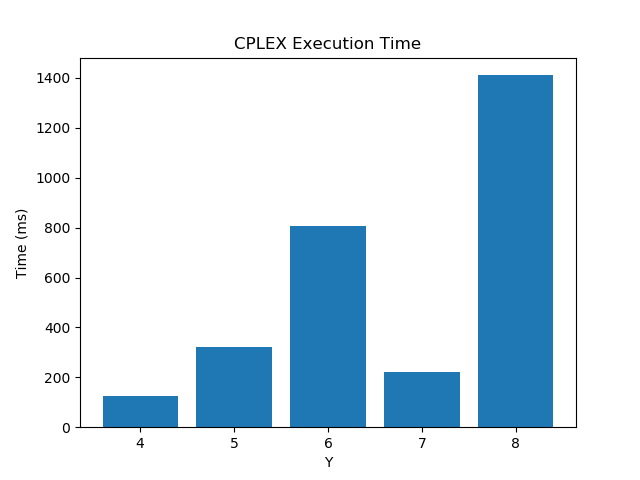
\includegraphics[width=0.8\textwidth]{cplex_data_time}
	\caption{The time taken to execute the LP file in CPLEX for each network.}
	\label{fig:cplex_time}
\end{figure}

\begin{figure}[H]
	\centering
	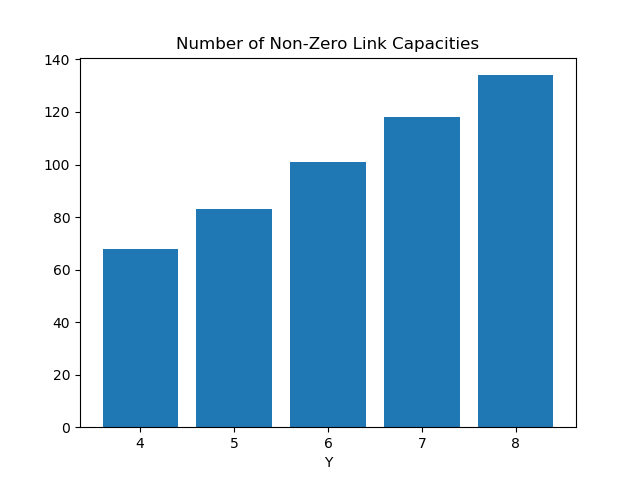
\includegraphics[width=0.8\textwidth]{cplex_data_num_nonzero_links}
	\caption{The number of non-zero link capacities in each network.}
	\label{fig:cplex_num_nonzero_links}
\end{figure}

\begin{figure}[H]
	\centering
	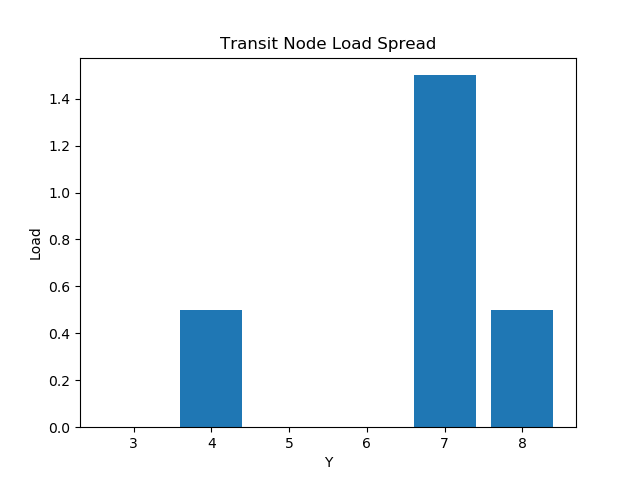
\includegraphics[width=0.8\textwidth]{cplex_data_transit_load_spread}
	\caption{The amount of spread in the load for all transit nodes in each network.}
	\label{fig:cplex_transit_load_spread}
\end{figure}

\begin{figure}[H]
	\centering
	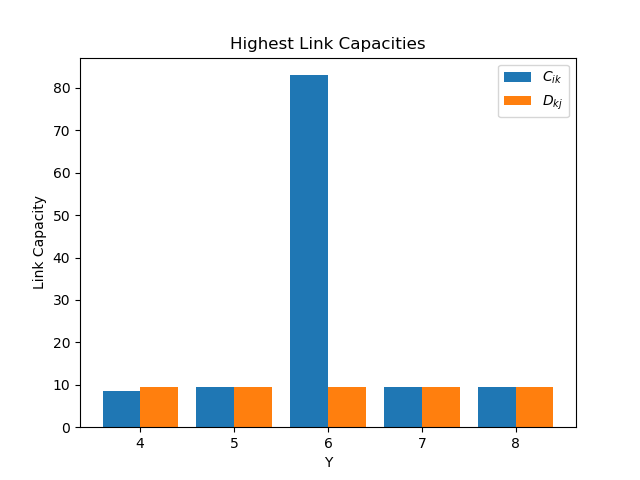
\includegraphics[width=0.8\textwidth]{cplex_data_highest_capacity_links}
	\caption{The highest capacity links for each network. Both the $c_{ik}$ and $d_{kj}$ links are listed.}
	\label{fig:cplex_highest_capacity_links}
\end{figure}

% Show results for the CPLEX execution time, the number of links with non-zero capacities, the spread of the transit node loads (the difference between the largest and the smallest transit node load), and the highest capacity links, for all varying Y.
% Show these results as a graph or a table.
% Please explain the results

\section{Appendix}


\subsection{Source Code}
\label{section:source}

\subsubsection{src/lp\_gen.py}
This script is responsible for producing a valid LP file from the given command line parameters.
\lstinputlisting[language=Python]{../src/lp_gen.py}

\subsubsection{src/lp\_csv.py}
This script is responsible for converting the output of the CPLEX log files into a single CSV file for further processing.
\lstinputlisting[language=Python]{../src/lp_csv.py}

\subsubsection{src/lp\_graph.py}
This script is responsible for reading the CSV file and producing several graphs.
\lstinputlisting[language=Python]{../src/lp_graph.py}

\subsubsection{output.sh}
This BASH script is responsible for executing the other scripts as well as timing and running CPLEX (under the Linux operating system).
\lstinputlisting[language=BASH]{../output.sh}

\subsubsection{output.ps1}
This PowerShell script is responsible for executing the other scripts as well as timing and running CPLEX (under the Windows operating system).
\lstinputlisting{../output.ps1}

\newpage

\subsection{Generated LP File}

\subsubsection{lp\_files/problem\_3\_2\_4.lp}
\lstinputlisting{../lp_files/problem_3_2_4.lp}

\end{document}
